%!TEX root = ../template.tex
%%%%%%%%%%%%%%%%%%%%%%%%%%%%%%%%%%%%%%%%%%%%%%%%%%%%%%%%%%%%%%%%%%%%
%% annex2.tex
%% NOVA thesis document file
%%
%% Chapter with example of appendix with a short dummy text
%%%%%%%%%%%%%%%%%%%%%%%%%%%%%%%%%%%%%%%%%%%%%%%%%%%%%%%%%%%%%%%%%%%%
\chapter{SGX Local Attestation}
\label{ann:sgx_local_attestation}

This annex contains the information that describes the Intel's \gls{SGX} local attestation process and the text was directly taken from \textit{sgx101.com} \cite{sgx:localAttestation}.

Before multiple enclaves collaborate with each other on the same platform, one enclave will have to authenticate the other locally using Intel SGX Report mechanism to verify that the counterpart is running on the same TCB platform by applying the REPORT based Diffie-Hellman Key Exchange. This procedure is referred as local attestation by Intel. The successful result of local attestation will offer a protected channel between two local enclaves with guarantee of confidentiality, integrity and replay protection.

\begin{figure}[htbp]
	\centerline{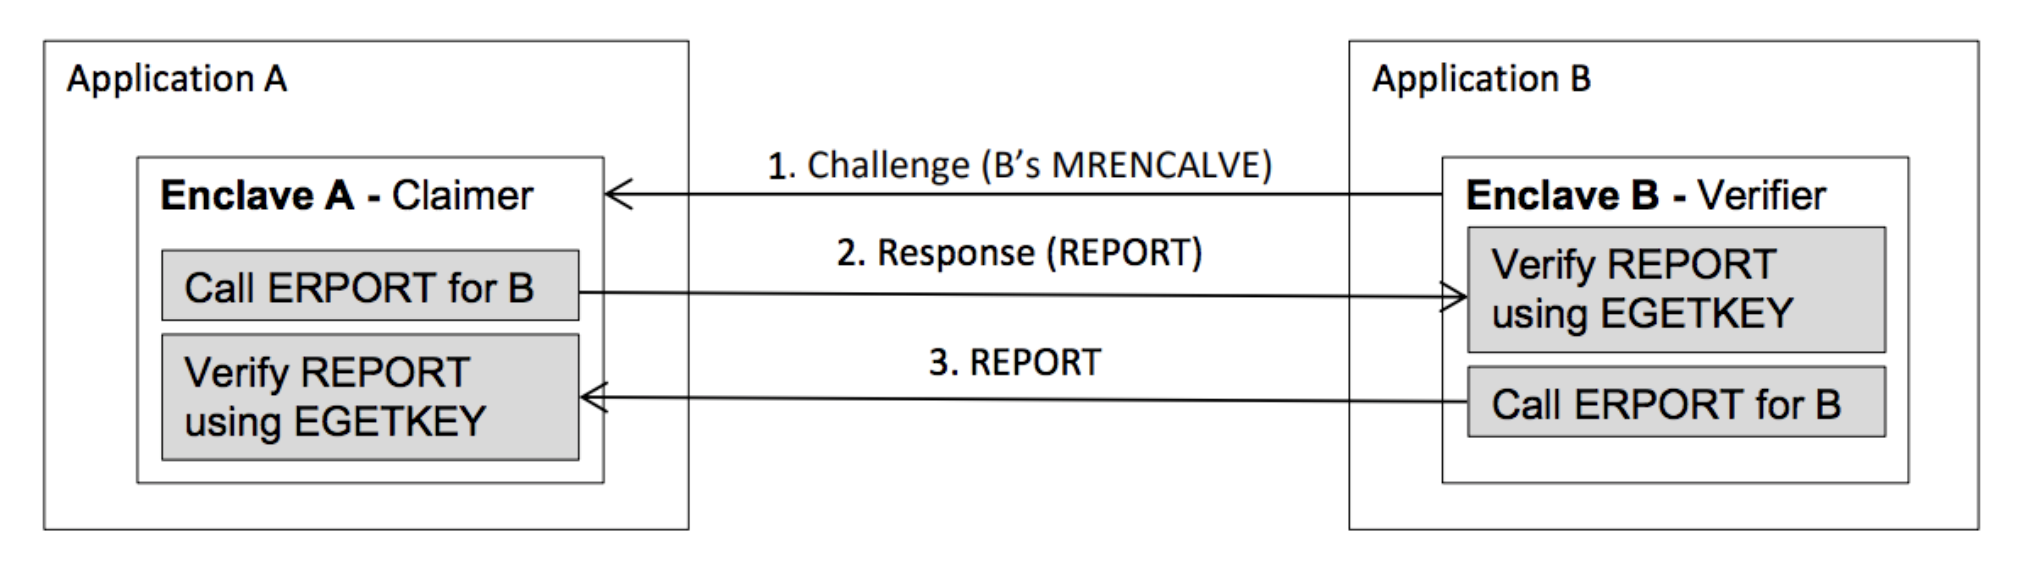
\includegraphics[width=0.99\linewidth]{sgx_local_attestation}}%
	\caption{SGX Local Attestation}
	\label{fig:sgx_local_attestation}
\end{figure}

There are two enclaves on the same platform, referred to as Enclave A and Enclave B. We assume they have established a communication path between each other, and the path doesn’t need to be trusted. W.l.o.g we assume B is asking A to prove it’s running on the same platform as B.

\begin{enumerate}
	\item First, B retrieves its MRENCLAVE value and sends it to A via the untrusted channel.
	\item A uses EREPORT instruction to produce a report for B using B’s MRENCLAVE. Then A sends this report back to B. A can also include Diffie-Hellman Key Exchange data in the REPORT as user data for trusted channel creation in the future.
	\item After B receives the REPORT from A, B calls EGETKEY instruction to get REPORT KEY to verify the REPORT. If the REPORT can be verified with the REPORT KEY, then B assures that A is on the same platform as B because the REPORT KEY is specific to the platform.
	\item Then B use the MRENCLAVE received from A’s REPORT to create another REPORT for A and sends the REPORT to A.
A then also can do the same as step 4 to verity B is on the same platform as A.
	\item A then also can do the same as step 4 to verity B is on the same platform as A.
	\item By utilising the user data field of the REPORT, A and B can create a secure channel using Diffie-Hellman Key Exchange. Information exchange can be encrypted by the shared symmetric key.
\end{enumerate}